\subsection{Revisiting Example~\ref{subsec:pde-example}}
Recall that aggregating spatial data into two separate components on $\qoi_\text{2D}$ provides a tangible benefit for resolving the uncertainty in the true function $g$ as seen in Example~\ref{subsec:pde-example}.
However, we did not present how the map $\qoi_\text{2D}$ was selected.
To explore the impact of various choices in how data may be aggregated into components of a QoI map, we propose two methods for splitting the measurements into two subsets to construct the respective components of the map according to \eqref{eq:qoi_WME}.
An illustration of the partitioning for both methods is shown in the top half of Figure~\ref{fig:pde-highd-2d-geometry}; a bisection of $\Omega$ into vertically-oriented halves is used to form $\qoi_\text{2D}^\prime$ and (as before) horizontal ones for $\qoi_\text{2D}$.

\begin{figure}
\centering
  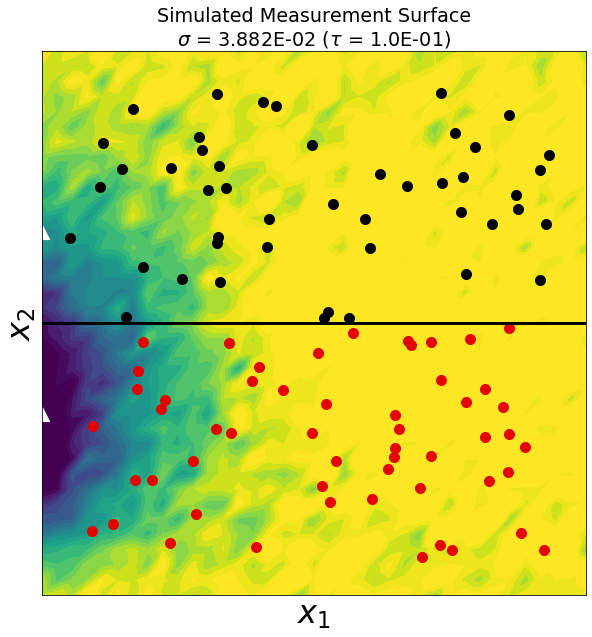
\includegraphics[width=0.475\linewidth]{figures/pde-highd/pde-highd_sensors_D2.png}
  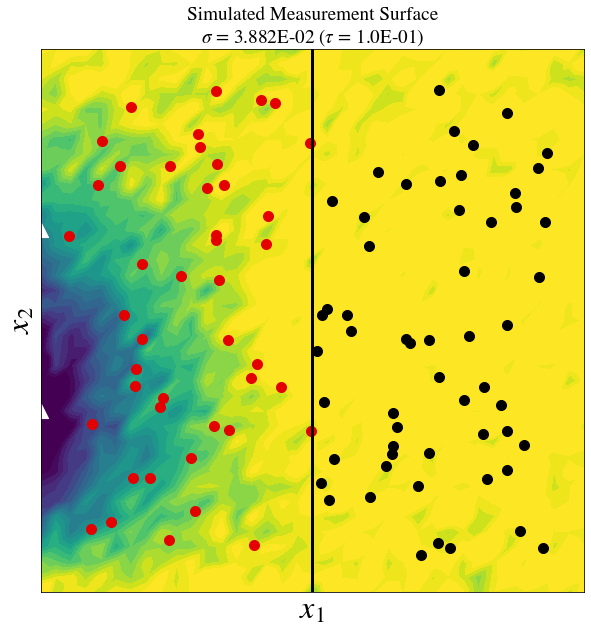
\includegraphics[width=0.475\linewidth]{figures/pde-highd/pde-highd_sensors-alt_D2.png}
  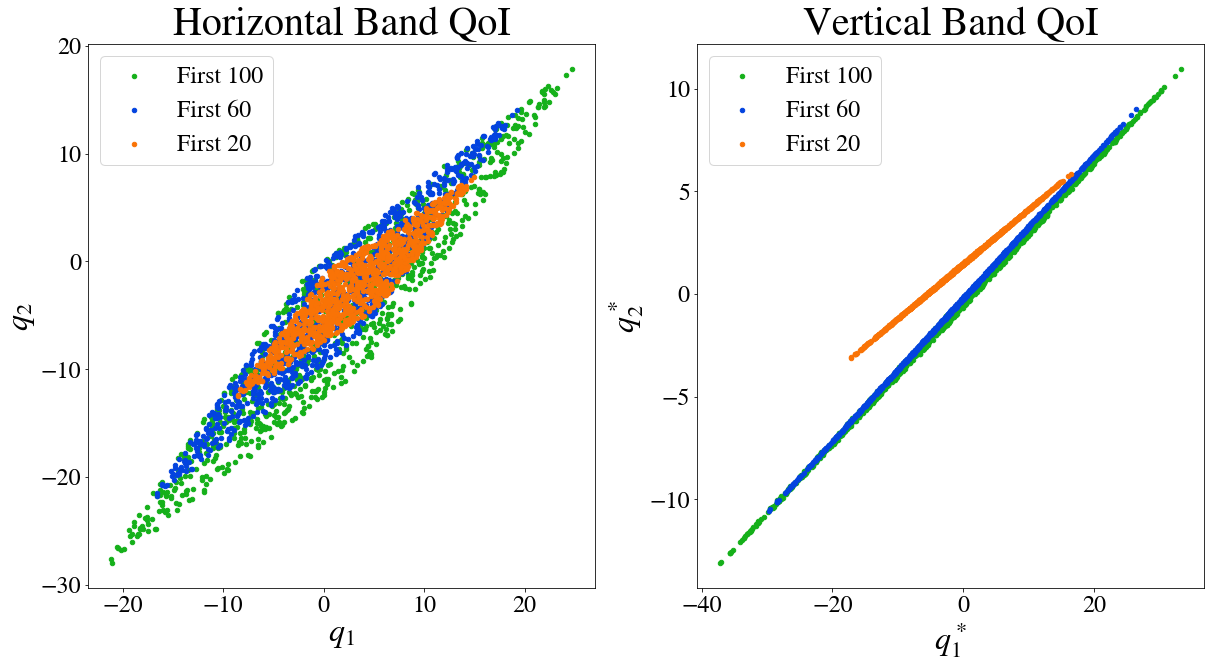
\includegraphics[width=0.95\linewidth]{figures/pde-highd/pde-highd_geom_D2.png}
\caption{
Comparison of $\qoi_\text{2D}$ (left) and $\qoi_\text{2D}^\prime$ (right).
Partitioning of $\Omega$ into the two components of each map is shown in the top half of the figure.
In the bottom half, the vector-valued QoI map is constructed for all $N=1000$ parameter evaluations using $\ndata=20, 60, \text{ and } 100$ measurements, and the two resulting component vectors are plotted against one another for both methods of partitioning $\Omega$.
}
\label{fig:pde-highd-2d-geometry}
\end{figure}

The choice of which partitioning method to use is akin to the following question:
\begin{center}
\emph{With two possible QoI maps under consideration, which should we use?}
\end{center}

We use heuristics and an understanding of skewness to help address this question.
For the data-constructed (WME) QoI map, the observed distribution for which we seek a pullback measure is fixed as a standard multivariate Gaussian, independent of the number of measurements that were used.
The initial density is also a fixed quantity, implying that any differences in the updated density will be attributed to differences in the predicted density.
To understand how the precision of the MUD estimate will change as more measurements are incorporated into the map, we visualize the data spaces induced by the WME QoI for increasing number of measurements $\ndata = 20, 60, \text{ and } 100$.

We sample the predicted data spaces using simulated spatial data associated with $1000$ parameter samples.
To build intuition about how the underlying geometry induced by these maps changes, we plot the scatter-plots representing a visualization of the associated data spaces in the bottom half of Figure~\ref{fig:pde-highd-2d-geometry}.
This figure also shows the associated designs against the noisy response surface as a backdrop.
The inclusion of more data points has the effect of dilating (and to some extent rotating) the induced data space for both QoI maps.
This dilation is expected based on Corollary~\ref{cor:MUD_wme} where it is established (for linear maps), that the predictability assumption is satisfied once enough data are obtained.

$\qoi_\text{2D}^\prime$ has much higher skewness than $\qoi_\text{2D}$, as is visually evident by the near-perfect correlation between its component values seen in the right plot of Fig~\ref{fig:pde-highd-2d-geometry}.
The most notable difference between the scatterplots is the difference in diameters (reference the axis labels) for each data space, a fact attributable to the difference in skewness.
The two component maps of $\qoi_\text{2D}^\prime$ contain almost the same information, so we can expect there to be little difference between MUD points arising from using $\qoi_\text{2D}^\prime$ when compared to using the scalar--valued map.
We compare these two solutions for an instance of the SIP in Figure~\ref{fig:pde-highd-2d-scalar-vs-alt}.

\begin{figure}
  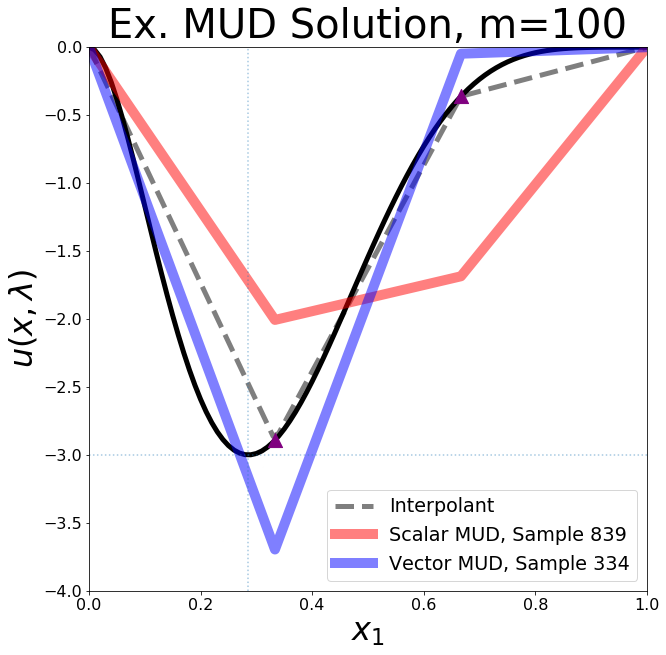
\includegraphics[width=0.95\linewidth]{figures/pde-highd/pde-highd_comp_exmud_D2_m100.png}
\caption{
Side-by-side comparison of an example solution to the SIP using $\qoi_\text{1D}$ (left) compared to using $\qoi_\text{2D}^\prime$, juxtaposed against a plot of $g$.
}
\label{fig:pde-highd-2d-scalar-vs-alt}
\end{figure}

By contrast, the map induced by a horizontal split (bottom left of Fig. \ref{fig:pde-highd-2d-geometry}) provides new information in each component.
While there is some correlation (the predicted data spaces are not rectangular), a far greater proportion of samples will fall within the practical support of the observed distribution, which qualifies them as possible solutions to the SIP.
More information is learned with the inclusion of each component using this design than would be with the vertical split.
Using a quantitative measure such as average skewness allows us to scale the assessment to higher-dimensional parameter and data spaces when visual inspection is not possible.

We focus attention on comparing higher-dimensional QoI maps constructed from aggregating data separated into more horizontal bands to scalar QoI maps (as proxies for highly-skewed maps), and note that a more thorough discussion of constructing QoI maps that induce desirable geometric properties is of interest for future work.
In \ref{sec:mud-higher-dimensions} and \ref{sec:mud-pde-sequence}, the ``vector--valued'' map will refer to the one with data aggregated into separate horizontal bands.
We note that this design, while not guaranteeing optimality for precision or accuracy's sake, respects the flow of information in the system being studied.
Since the parameter represents the left Neumann boundary condition, information about its state flows from left to right in the horizontal direction.

\FloatBarrier
